\newpage

\section*{\centerline{Цель работы}}

Получение навыков работы с командной строкой UNIX и UNIX-подобных систем, а также навыки работы с каталогами, папками и дисками в GNU/Linux. Изучить основные команды и утилиты GNU/Linux. 
\newpage

\section*{\centerline{Выполнение}}
\vspace{1cm}

\subsection*{\centerline{Задание 1.1}}
\vspace{0.5cm}
\subsection*{Описание работы основных программ:}
Для того чтобы получить описание команд, параметров и ключей необходимо написать \textit{man 'command'} или \textit{'command' --help}
\vspace{0.5cm}

Команда \textit{nano} открывает консольный текстовый редактор.
\begin{figure}[h!]
\centering
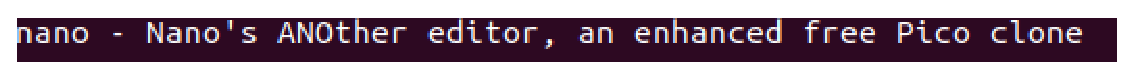
\includegraphics [width=\textwidth]{mnano.eps}\\
\end{figure}
\\

Команда \textit{mv} позволяет перемещать и переименовывать файлы и папки.
\begin{figure}[h!]
\centering
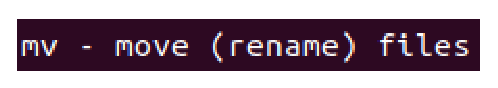
\includegraphics [width=\textwidth]{mmv.eps}\\
\end{figure}
\\

Команда \textit{rm} позволяет удалить файл или папку.
\begin{figure}[h!]
\centering
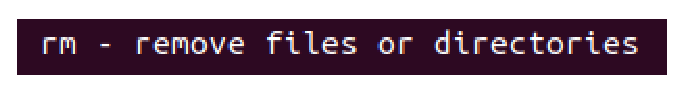
\includegraphics [width=\textwidth]{mrm.eps}\\
\end{figure}
\\

Команда \textit{df} отображает пути и названия смонтированных разделов и дисков.
\begin{figure}[h!]
\centering
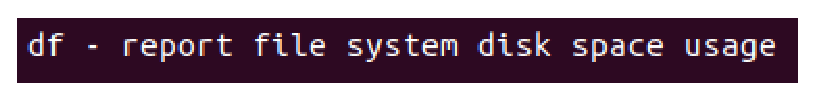
\includegraphics [width=\textwidth]{mdf.eps}\\
\end{figure}
\\

Команда \textit{du} вес папок и файлов(по умолчанию в KiB).
\begin{figure}[h!]
\centering
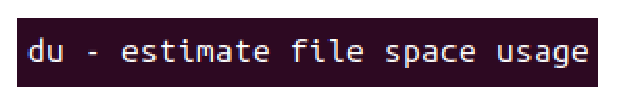
\includegraphics [width=\textwidth]{mdu.eps}\\
\end{figure}
\\

Команда \textit{free} показывает текушее состояние оперативной памяти(доступность, занятость системой и зарезервированность)
\begin{figure}[h!]
\centering
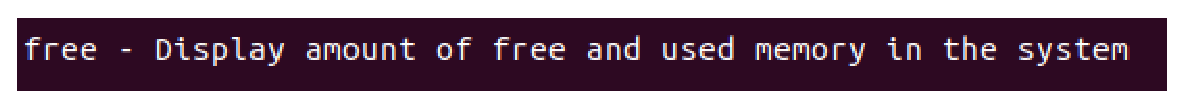
\includegraphics [width=\textwidth]{mfree.eps}\\
\end{figure}
\\
\newpage

Команда \textit{top} показывает нагруженность системы, позволяет управлять процессами и задачами(завершать и менять проиоритет)
\begin{figure}[h!]
\centering
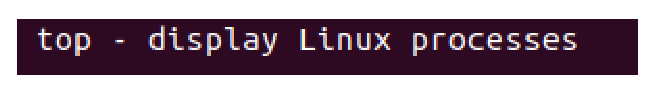
\includegraphics [width=\textwidth]{mtop.eps}\\
\end{figure}
\\

Команда \textit{ls} показывает список файлов и папок в данной директории, права, вес и дату создания(с ключиком -l)
\begin{figure}[h!]
\centering
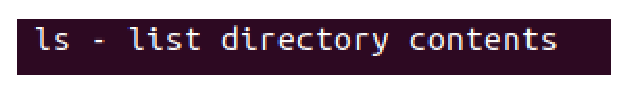
\includegraphics [width=\textwidth]{mls.eps}\\
\end{figure}
\\

Команда \textit{pwd} показывает текущее местоположение.
\begin{figure}[h!]
\centering
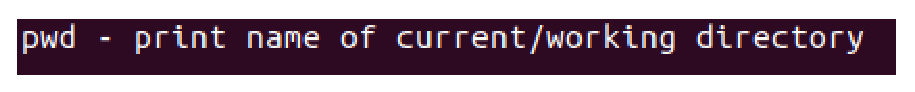
\includegraphics [width=\textwidth]{mpwd.eps}\\
\end{figure}
\\

Команда \textit{clear} очищает консоль.
\begin{figure}[h!]
\centering
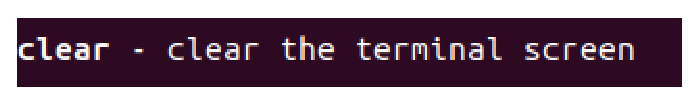
\includegraphics [width=\textwidth]{mclear.eps}\\
\end{figure}
\\

Команда \textit{uname} выводит имя релиза системы, версию ядра Linux и название дистрибутива(дату создания)
\begin{figure}[h!]
\centering
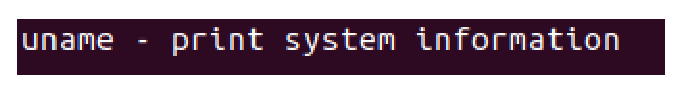
\includegraphics [width=\textwidth]{muname.eps}\\
\end{figure}
\\

Команда \textit{man} отображает мануал по выбранной функции
\begin{figure}[h!]
\centering
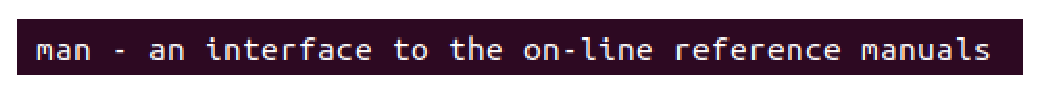
\includegraphics [width=\textwidth]{mman.eps}\\
\end{figure}
\\

Команда \textit{lsmod} показывает системные модули(драйвера) и их размер.
\begin{figure}[h!]
\centering
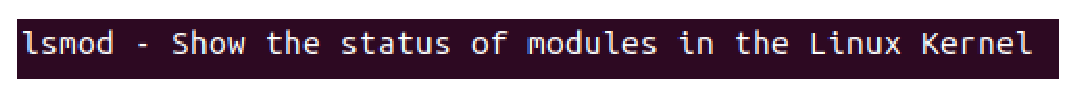
\includegraphics [width=\textwidth]{mlsmod.eps}\\
\end{figure}
\\

\newpage
Команда \textit{date} отображает текущую дату и часовой пояс.
\begin{figure}[h!]
\centering
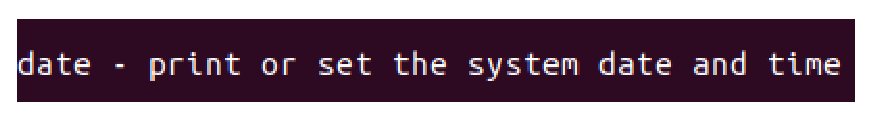
\includegraphics [width=\textwidth]{mdate.eps}\\
\end{figure}

\vfill
\newpage

\subsection*{Задание 1.1(a) Показать нагруженность системы.}
Была выбрана команда \textit{htop}, поскольку она выводит больший(по сравнению с \textit{top}) перечень процессов и свойств нагруженности системы, обладаем элементами выборочной сортировки.
Также \textit{top} и \textit{htop} отображают текущую нагрузку на ядра процессора, среднюю нагрузку за разные интервалы времени. Обьем занятой оперативной памяти, swap и количество активных задач и процессов\\
\\
\begin{figure}[h!]
\centering
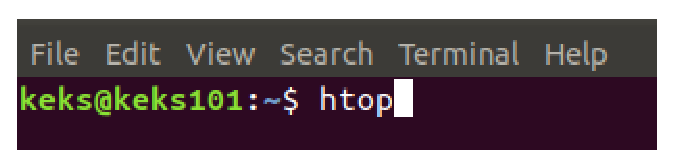
\includegraphics [width=\textwidth]{htop0.eps}\\
\end{figure}
\begin{figure}[h!]
\centering
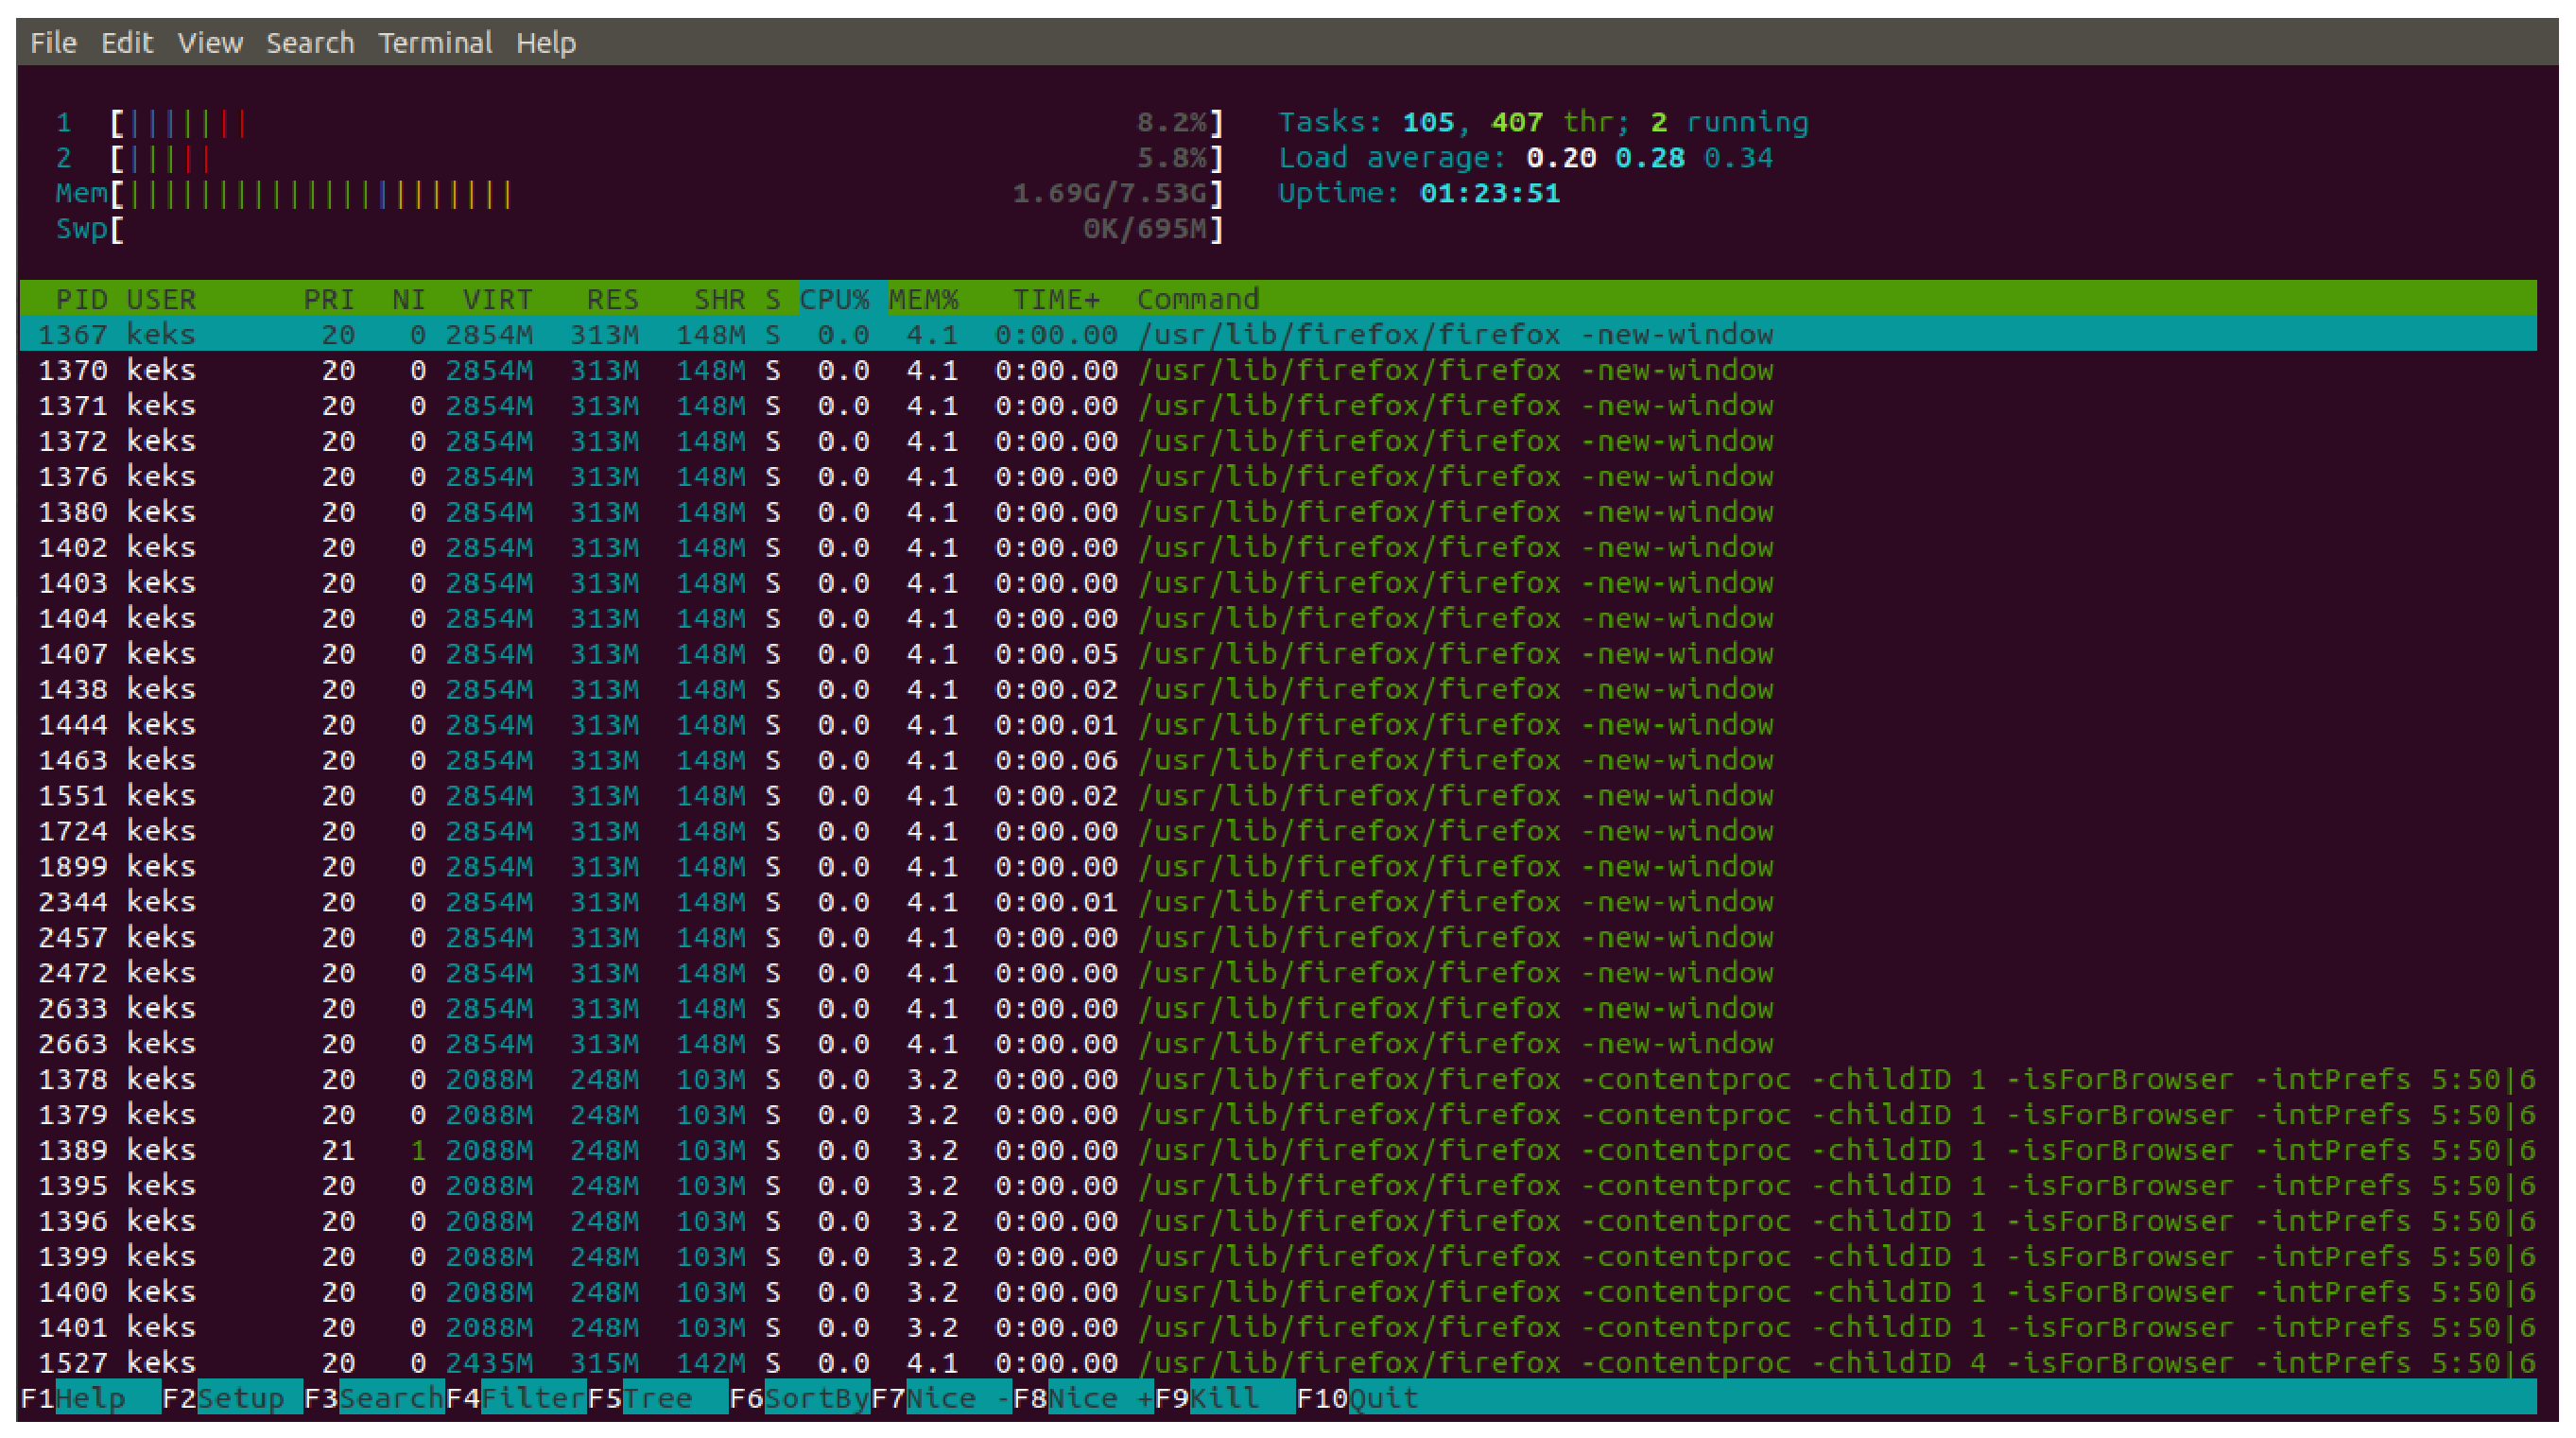
\includegraphics [width=\textwidth]{htop.eps}\\
\end{figure}

\newpage

\subsection*{Задание 1.1(b) Отобразить объем занятой оперативной памяти в килобайтах.}
Была выбрана команда free соответственно с ключом \textit{--kilo} или его сокращенной версией \textit{-k}.
Здесь занятую оперативную память в килобайтах показывает число под графой \textit{used}.

\begin{figure}[h!]
\centering
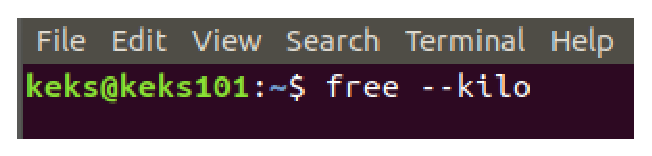
\includegraphics [width=1\textwidth]{free0.eps}\\
\end{figure}
\begin{figure}[h!]
\centering
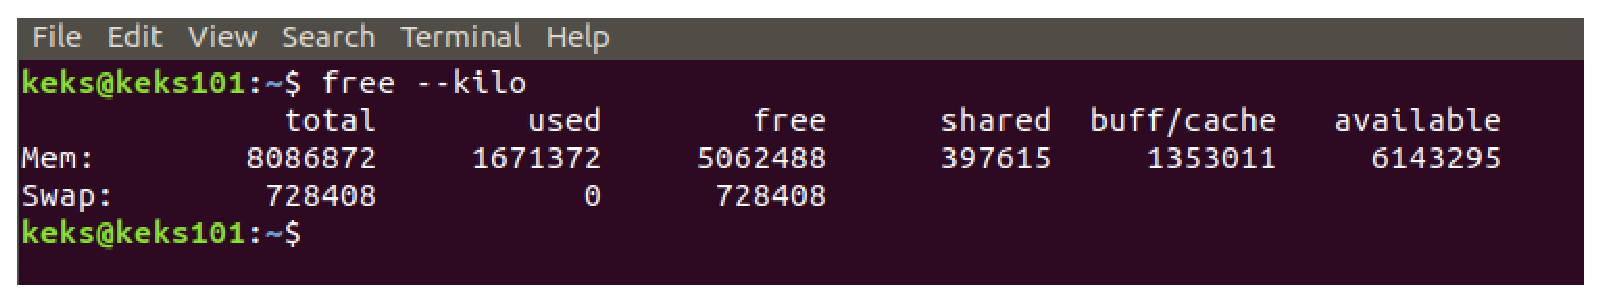
\includegraphics [width=1\textwidth]{free.eps}\\
\end{figure}